From the given information, since the 
slope of the line is 1, 
\begin{align}
        \vec{m}&=\myvec{1\\1},  c=1
\\
 \implies \vec{n}=  \myvec{-1\\1}     
\end{align}
and the equation of the line is given by

\begin{align}
\myvec{-1&1}\vec{x} =1     
\end{align}
%
plotted in Fig. \ref{5/1/fig}.
%
\begin{figure}[!ht]
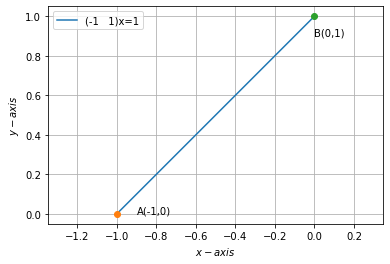
\includegraphics[width=\columnwidth]{Line.png}
\caption{ Plot of a straight line  }
\label{5/1/fig}
\end{figure}

